Pour pouvoir transmettre les messages depuis l'utilisateur vers le téléphone portable, nous avons
choisi de mettre en place un site web à l'allure d'un gestionnaire de conversation. 
blablabla

Le fonctionnement de ce projet repose grandement sur la partie qui suit.
\\


%%%%%%%%%%%%%%%%%%%%%%%%%%%%%%%%%%%%%%%%%%%%%%%%%%%%%%%%%%%%%%%%%%%%%%%%%%%%%%%%%%%%%%%%%%%%%%%%%%%%
\subsection{Play Framework 2.0}
%%%%%%%%%%%%%%%%%%%%%%%%%%%%%%%%%%%%%%%%%%%%%%%%%%%%%%%%%%%%%%%%%%%%%%%%%%%%%%%%%%%%%%%%%%%%%%%%%%%%

\subsubsection{Primefaces vs Play Framework}



%%%%%%%%%%%%%%%%%%%%%%%%%%%%%%%%%%%%%%%%%%%%%%%%%%%%%%%%%%%%%%%%%%%%%%%%%%%%%%%%%%%%%%%%%%%%%%%%%%%%
\subsection{Authentification avec OAuth 2.0} % voir si l'on ne peut pas factoriser du rapport avec la partie Androïd
%%%%%%%%%%%%%%%%%%%%%%%%%%%%%%%%%%%%%%%%%%%%%%%%%%%%%%%%%%%%%%%%%%%%%%%%%%%%%%%%%%%%%%%%%%%%%%%%%%%%



%%%%%%%%%%%%%%%%%%%%%%%%%%%%%%%%%%%%%%%%%%%%%%%%%%%%%%%%%%%%%%%%%%%%%%%%%%%%%%%%%%%%%%%%%%%%%%%%%%%%
\subsection{Gestion des contacts}
%%%%%%%%%%%%%%%%%%%%%%%%%%%%%%%%%%%%%%%%%%%%%%%%%%%%%%%%%%%%%%%%%%%%%%%%%%%%%%%%%%%%%%%%%%%%%%%%%%%%

La gestion des contacts de l'utilisateur est un point important de notre cahier des charges.
\\

\subsubsection{Téléchargement des contacts Google}

\subsubsection{Tri et Formatage}

\subsubsection{Google cache}




%%%%%%%%%%%%%%%%%%%%%%%%%%%%%%%%%%%%%%%%%%%%%%%%%%%%%%%%%%%%%%%%%%%%%%%%%%%%%%%%%%%%%%%%%%%%%%%%%%%%
\subsection{Envoi des messages avec les websockets}
%%%%%%%%%%%%%%%%%%%%%%%%%%%%%%%%%%%%%%%%%%%%%%%%%%%%%%%%%%%%%%%%%%%%%%%%%%%%%%%%%%%%%%%%%%%%%%%%%%%%



\subsubsection{websocket}

\subsubsection{notification}



%%%%%%%%%%%%%%%%%%%%%%%%%%%%%%%%%%%%%%%%%%%%%%%%%%%%%%%%%%%%%%%%%%%%%%%%%%%%%%%%%%%%%%%%%%%%%%%%%%%%
\subsection{Design du site}
%%%%%%%%%%%%%%%%%%%%%%%%%%%%%%%%%%%%%%%%%%%%%%%%%%%%%%%%%%%%%%%%%%%%%%%%%%%%%%%%%%%%%%%%%%%%%%%%%%%%

Le design du site est l'un des thèmes que nous avons travaillé pour cette partie la du projet.

Nous souhaitions initialement avoir une interface simple, sans fioritures car cela nous semblait comme
secondaire. Nous avons donc utilisé deux frameworks pour nous faciliter la tache et accélérer la mise
en place du design.

Nous avons donc tout d'abord choisi "Twitter Bootstrap" puis nous l'avons couplé au framework "jQuery
Layout".
\\


\subsubsection{Twitter Bootstrap}

\textit{Twitter Bootstrap}\footnote{Site web : \href{http://twitter.github.com/bootstrap/}{http://twitter.github.com/bootstrap/}} est un framework web utilisé pour le développement front end.
C'est un outil écrit en JavaScript et CSS qui permet de réaliser facilement des interfaces élégantes néanmoins simples. 

Il nous a été utile principalement pour pouvoir concevoir l'affichage des zones d'entrée de textes ou 
encore pour organiser l'affichage des contacts proprement.
\\


\subsubsection{jQuery Layout}

\textit{jQuery Layout}\footnote{Site web : \href{http://layout.jquery-dev.net/}{http://layout.jquery-dev.net/}} est aussi un framework web qui, contrairement à Twitter Bootstrap, permet d'organiser les sites en plusieurs interfaces distinctes. 
L'utilité de JQuery Layout réside dans sa possibilité à fractionner un espace en plusieurs fenêtres.
Cela permet de retrouver l'ergonomie et le coté simple et ordonné des logiciels. 

Ce framework très riche nous a donc été très profitable pour pouvoir obtenir une bonne ergonomie sans avoir
à trop passer du temps sur cette partie.
Le schéma \ref{siteWeb_jQueryLayout} représente l'agencement général de notre site web grâce à ce framework.

\begin{figure}[!h]
	\center
	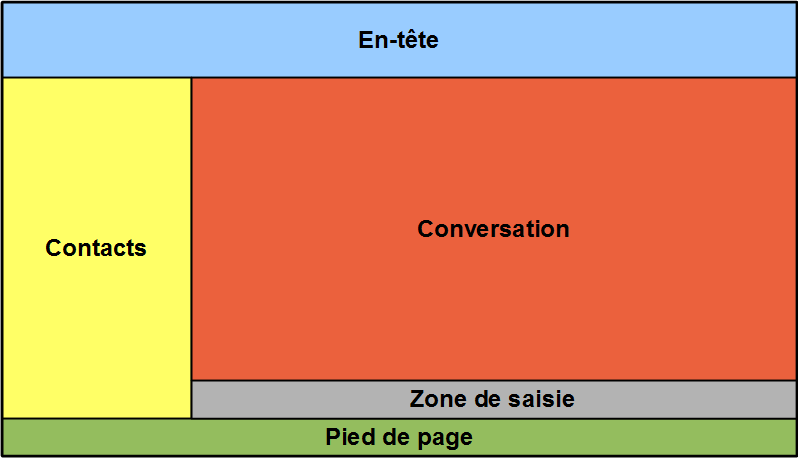
\includegraphics[width=13cm]{img/siteWeb_jQueryLayout.png}
	\caption{jQuery Layout : structure du site web}
	\label{siteWeb_jQueryLayout}
~~\\
\end{figure}




%\begin{figure}[!h]
%	\center
%	\includegraphics[width=13cm]{img/.png}
%	\caption{}
%	\label{}
%\end{figure}
